\section{覆叠空间的存在性}
\label{ch13-sec82}

我们已经证明了每一个覆叠映射 $p\colon E\to B$ 对应着 $\pi_{1}(B,\ b_{0})$ 的子群的一个共轭类, 并且证明了两个覆叠映射等价的充分必要条件是它们对应着相同的这种类. 因此, 我们已经得到了由 $B$ 的覆叠映射的等价类到 $\pi_{1}(B,\ b_{0})$ 的子群的共轭类间的一个单射. 现在, 我们提出以下问题: 上述对应是否是一个满射? 也就是说, 对于 $\pi_{1}(B,\ b_{0})$ 的子群的每一个共轭类, 是否存在 $B$ 的一个覆叠映射与之对应?

一般来说, 回答是否定的. 在第 80 节中, 我们曾经给出一个例子, 在那里 $B$ 是一个道路连通且局部道路连通的空间, 它没有单连通的覆叠空间, 也就是说, 没有覆叠空间对应着平凡子群的共轭类. 这个例子依赖于 \cref{lemma:ch13-simply-connected-local-trivial}, 这个引理给出了任何一个空间有单连通的覆叠空间时所必须满足的条件. 现在我们将这个条件陈述如下.

\begin{definition}[半局部单连通]
\label{definition:ch13-semilocally-simply-connected}
称空间 $B$ 为\textbf{半局部单连通的}(semilocally simply connected), 如果对于每一个 $b\in B$, 存在 $b$ 的一个邻域 $U$ 使得由内射诱导的同胚
\[
i_{*}\colon\pi_{1}(U,b)\longrightarrow\pi_{1}(B,b)
\]
是平凡的.
\end{definition}

注意当 $U$ 满足上述条件时, $b$ 的任意较小的邻域也满足上述条件, 所以 $b$ 有"任意小"的邻域满足这个条件. 此外, 上述条件要弱于真正的局部单连通性, 因为局部单连通性意指 $b$ 的每一邻域包含着 $b$ 的某一个单连通的邻域 $U$.

$B$ 是半局部单连通的当且仅当基本群 $\pi_{1}(B,\ b_{0})$ 的子群的每一个共轭类存在一个 $B$ 的覆叠空间与之对应. 必要性已经在 \cref{lemma:ch13-simply-connected-local-trivial} 中证明了, 本节将给出充分性的证明.

\begin{theorem}[覆叠空间的存在性]
\label{theorem:ch13-covering-existence}
设 $B$ 是道路连通、局部道路连通且半局部单连通的. 令 $b_{0}\in B$. 则对于 $\pi_{1}(B,\ b_{0})$ 中任意给定的一个子群 $H$, 存在一个覆叠映射 $p\colon E\to B$ 以及点 $e_{0}\in p^{-1}(b_{0})$ 使得
\[
p_{*}(\pi_{1}(E,e_{0}))=H.
\]
\end{theorem}

\par
\begin{figure}[htbp]
\centering
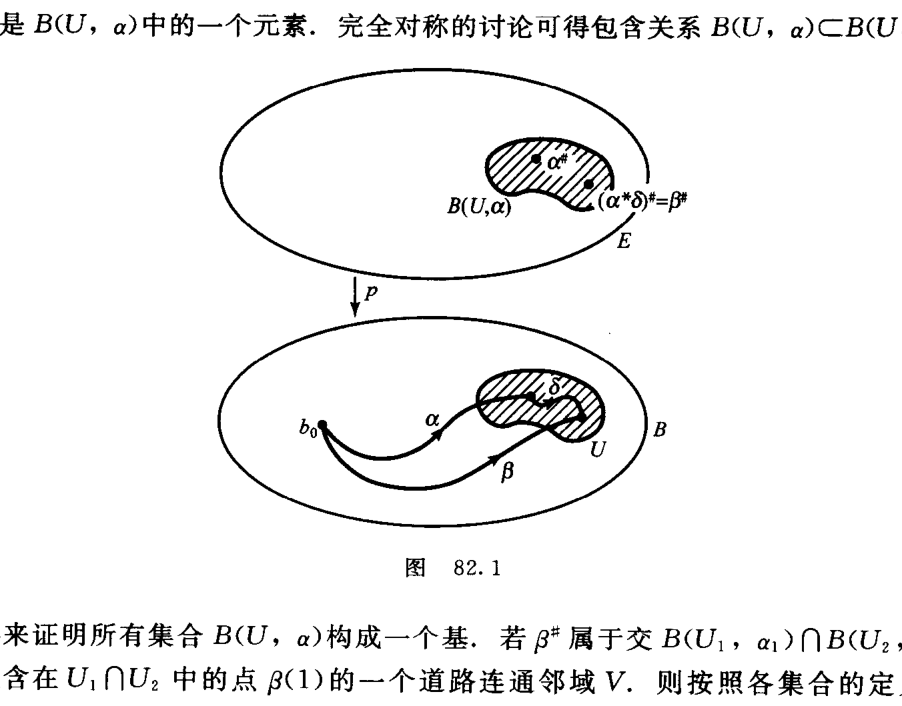
\includegraphics[width=0.6\textwidth]{image/fig-82-1.png}
\caption{覆叠空间 $E$ 的构造.}
\label{ch13-fig-82-1}
\end{figure}

\par
\begin{figure}[htbp]
\centering
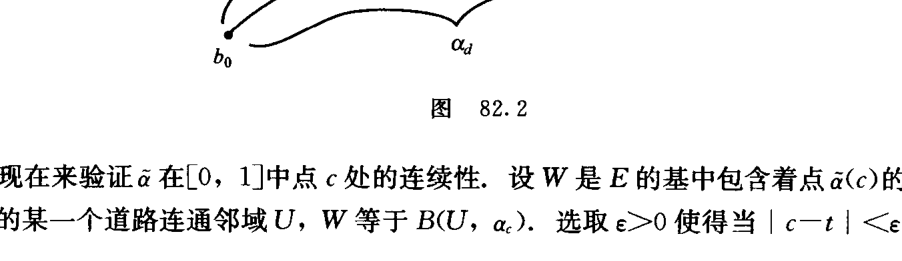
\includegraphics[width=0.7\textwidth]{image/fig-82-2.png}
\caption{道路的提升.}
\label{ch13-fig-82-2}
\end{figure}

\begin{proof}
\textbf{第一步. $E$ 的构造.} $E$ 的构造过程与复分析中构造 Riemann 曲面的过程完全相仿. 设 $\mathcal{P}$ 表示 $B$ 中所有以 $b_{0}$ 为起点的道路的集合. 在 $\mathcal{P}$ 上定义等价关系如下: 若 $\alpha$ 和 $\beta$ 在 $B$ 中有相同的终点并且
\[
[\alpha*\overline{\beta}]\in H,
\]
则规定 $\alpha\sim\beta$. 容易验证, 这是一个等价关系. 我们将用 $\alpha^{\#}$ 表示 $\alpha$ 的等价类.

设 $E$ 为所有等价类的集合. 通过关系式
\[
p(\alpha^{\#})=\alpha(1)
\]
定义映射 $p\colon E\to B$. 由于 $B$ 是道路连通的, 所以 $p$ 是满射. 我们将赋予 $E$ 一个拓扑使得 $p$ 为覆叠映射.

首先注意以下两个事实:
\begin{enumerate}[(1)]
\item 若 $[\alpha]=[\beta]$, 则 $\alpha^{\#}=\beta^{\#}$.
\item 若 $\alpha^{\#}=\beta^{\#}$, 则 $(\alpha*\delta)^{\#}=(\beta*\delta)^{\#}$, 其中 $\delta$ 为 $B$ 中任何一条以 $\alpha(1)$ 为起点的道路.
\end{enumerate}
前者成立是由于若 $[\alpha]=[\beta]$, 则 $[\alpha*\overline{\beta}]$ 为 $H$ 中的单位元. 后者成立是由于 $\alpha*\delta$ 和 $\beta*\delta$ 有相同的终点, 并且根据假设有
\[
[(\alpha*\delta)*\overline{(\beta*\delta)}]=[(\alpha*\delta)*(\overline{\delta}*\overline{\beta})]=[\alpha*\overline{\beta}]
\]
属于 $H$.

\textbf{第二步. $E$ 的拓扑化.} $E$ 的拓扑化的方式之一是在 $\mathcal{P}$ 上赋子紧开拓扑 (参见第 7 章) 并且在 $E$ 上取相应的商拓扑. 然而, 我们可以通过以下方法直接拓扑化 $E$:

设 $\alpha$ 是 $\mathcal{P}$ 中的任意一个元素, $U$ 为 $\alpha(1)$ 的任何一个道路连通的邻域. 定义
\[
B(U,\alpha)=\{(\alpha*\delta)^{\#}\mid\delta\text{ 是 }U\text{ 中一条以 }\alpha(1)\text{ 为起点的道路}\}.
\]
注意 $\alpha^{\#}$ 是 $B(U,\ \alpha)$ 中的一个元素. 这是因为: 若 $b=\alpha(1)$, 则 $\alpha^{\#}=(\alpha*e_{b})^{\#}$, 并且根据定义这是 $B(U,\ \alpha)$ 中的一个元素. 我们断言: 所有集合 $B(U,\ \alpha)$ 构成 $E$ 的某一个拓扑的基.

首先我们证明: 若 $\beta^{\#}\in B(U,\ \alpha)$, 则有 $\alpha^{\#}\in B(U,\ \beta)$ 和 $B(U,\ \alpha)=B(U,\ \beta)$.

如果 $\beta^{\#}\in B(U,\ \alpha)$, 则对于 $U$ 中的某条道路 $\delta$ 有 $\beta^{\#}=(\alpha*\delta)^{\#}$. 因此
\[
(\beta*\overline{\delta})^{\#}=((\alpha*\delta)*\overline{\delta})^{\#}=\alpha^{\#},
\]
从而根据定义有 $\alpha^{\#}\in B(U,\ \beta)$. 参见\cref{ch13-fig-82-1}. 我们先来证明 $B(U,\ \beta)\subset B(U,\ \alpha)$. 注意 $B(U,\ \beta)$ 的元素可表示为 $(\beta*\gamma)^{\#}$ 形式, 其中 $\gamma$ 是 $U$ 中的一条道路. 于是
\[
(\beta*\gamma)^{\#}=((\alpha*\delta)*\gamma)^{\#}=(\alpha*(\delta*\gamma))^{\#},
\]
根据定义这是 $B(U,\ \alpha)$ 中的一个元素. 完全对称的讨论可得包含关系 $B(U,\ \alpha)\subset B(U,\ \beta)$.


我们再来证明所有集合 $B(U,\ \alpha)$ 构成一个基. 若 $\beta^{\#}$ 属于交 $B(U_{1},\ \alpha_{1})\cap B(U_{2},\ \alpha_{2})$, 我们只需选取包含在 $U_{1}\cap U_{2}$ 中的点 $\beta(1)$ 的一个道路连通邻域 $V$. 则按照各集合的定义可见包含关系
\[
B(V,\beta)\subset B(U_{1},\beta)\cap B(U_{2},\beta)
\]
成立, 并且前面已经证明了上式右边的集合等于 $B(U_{1},\ \alpha_{1})\cap B(U_{2},\ \alpha_{2})$.

\textbf{第三步. $p$ 是一个连续开映射.} 为了证明 $p$ 是一个开映射, 我们只要证明基中的元素 $B(U,\ \alpha)$ 的像是 $B$ 中的开子集 $U$ 即可: 任意给定 $x\in U$, 选取 $U$ 中从 $\alpha(1)$ 到 $x$ 的一条道路 $\delta$, 则 $(\alpha*\delta)^{\#}$ 在 $B(U,\ \alpha)$ 中并且 $p((\alpha*\delta)^{\#})=x$.

为了证明 $p$ 的连续性, 选取 $E$ 中的一个元素 $\alpha^{\#}$ 以及 $p(\alpha^{\#})$ 的一个邻域 $W$. 选取集合 $W$ 中的点 $p(\alpha^{\#})=\alpha(1)$ 的一个道路连通邻域 $U$. 这时 $B(U,\ \alpha)$ 是 $\alpha^{\#}$ 的一个邻域, 并且 $p$ 将其映入 $W$ 中. 于是 $p$ 在 $\alpha^{\#}$ 处连续.

\textbf{第四步. $B$ 的每一点有一个邻域被 $p$ 均衡地覆盖着.} 给定 $b_{1}\in B$, 选取 $b_{1}$ 的一个道路连通邻域 $U$ 使得由内射所诱导的同态 $\pi_{1}(U,\ b_{1})\to\pi_{1}(B,\ b_{1})$ 是平凡的. 我们断言 $U$ 被 $p$ 均衡地覆盖着.

首先, 我们证明 $p^{-1}(U)$ 等于所有集合 $B(U,\ \alpha)$ 的并, 其中 $\alpha$ 取遍 $B$ 中所有从 $b_{0}$ 到 $b_{1}$ 的道路. 由于 $p$ 将每一个集合 $B(U,\ \alpha)$ 映到 $U$ 上, 显然 $p^{-1}(U)$ 包含这个并. 另一方面, 若 $\beta^{\#}$ 属于 $p^{-1}(U)$, 则 $\beta(1)\in U$. 在 $U$ 中选取从 $b_{1}$ 到 $\beta(1)$ 的一条道路 $\delta$ 并且设 $\alpha$ 是从 $b_{0}$ 到 $b_{1}$ 的道路 $\beta*\overline{\delta}$, 则 $[\beta]=[\alpha*\delta]$, 从而 $\beta^{\#}=(\alpha*\delta)^{\#}$, 它是 $B(U,\ \alpha)$ 中的一个元素. 于是 $p^{-1}(U)$ 包含于这些集合 $B(U,\ \alpha)$ 的并之中.

其次, 注意两个不同的形如 $B(U,\ \alpha)$ 的集合是无交的. 因为根据第二步可见, 当 $\beta^{\#}$ 属于 $B(U,\ \alpha_{1})\cap B(U,\ \alpha_{2})$ 时, $B(U,\ \alpha_{1})=B(U,\ \beta)=B(U,\ \alpha_{2})$.

最后, 我们证明 $p$ 是从 $B(U,\ \alpha)$ 到 $U$ 的一个一一映射. 由此推出 $p|B(U,\ \alpha)$ 是一个同胚, 即一一的连续开映射. 我们已知道 $p$ 将 $B(U,\ \alpha)$ 映满 $U$. 为了证明 $p$ 是一个单射, 假设
\[
p((\alpha*\delta_{1})^{\#})=p((\alpha*\delta_{2})^{\#}),
\]
其中 $\delta_{1}$ 与 $\delta_{2}$ 是 $U$ 中的两条道路. 这时有 $\delta_{1}(1)=\delta_{2}(1)$. 由于由内射诱导的同态 $\pi_{1}(U,\ b_{1})\to\pi_{1}(B,\ b_{1})$ 是平凡的, $\delta_{1}*\overline{\delta_{2}}$ 在 $B$ 中道路同伦于一条常值回路. 从而 $[\alpha*\delta_{1}]=[\alpha*\delta_{2}]$, 于是 $(\alpha*\delta_{1})^{\#}=(\alpha*\delta_{2})^{\#}$. 这便是我们要证明的.

由此可见 $p\colon E\to B$ 按照前几章中的说法是一个覆叠映射. 为了证明 $p$ 按照本章中的说法也是一个覆叠映射, 我们还要证明 $E$ 是道路连通的. 简要证明如下.

\textbf{第五步. 在 $B$ 中提升一条道路.} 设 $e_{0}$ 表示点 $b_{0}$ 处的常值道路的等价类, 则根据定义 $p(e_{0})=b_{0}$. 给定 $B$ 中以 $b_{0}$ 为起点的一条道路 $\alpha$, 我们来给出在 $E$ 中以 $e_{0}$ 为起点的一条道路作为它的提升, 并且证明这个提升以 $\alpha^{\#}$ 为终点.

为此, 给定 $c\in[0,\ 1]$, 并且设 $\alpha_{c}\colon I\to B$ 表示由
\[
\alpha_{c}(t)=\alpha(tc),\qquad\text{其中 }0\leq t\leq 1
\]
所定义的道路. 则 $\alpha_{c}$ 是 $\alpha$ 中从 $\alpha(0)$ 到 $\alpha(c)$ 的那一"段". 特别地, $\alpha_{0}$ 便是 $b_{0}$ 处的常值道路, 而 $\alpha_{1}$ 便是 $\alpha$ 本身. 我们用
\[
\widetilde{\alpha}(c)=(\alpha_{c})^{\#}
\]
定义 $\widetilde{\alpha}\colon I\to E$, 并且证明 $\widetilde{\alpha}$ 的连续性. 这时 $\widetilde{\alpha}$ 便是 $\alpha$ 的一个提升, 这是由于 $p(\widetilde{\alpha}(c))=\alpha_{c}(1)=\alpha(c)$, 从而, $\widetilde{\alpha}$ 以 $(\alpha_{0})^{\#}=e_{0}$ 为起点、以 $(\alpha_{1})^{\#}=\alpha^{\#}$ 为终点.

为了验证连续性, 我们引入以下记号. 给定 $0\leq c<d\leq 1$, 设 $\delta_{c,d}$ 表示由 $I$ 到 $[c,\ d]$ 的正线性映射与 $\alpha$ 的复合所定义的道路. 注意道路 $\alpha_{d}$ 和 $\alpha_{c}*\delta_{c,d}$ 是道路同伦的, 因为其中之一是另一个的再次参数化. 参见\cref{ch13-fig-82-2}.


我们现在来验证 $\widetilde{\alpha}$ 在 $[0,\ 1]$ 中点 $c$ 处的连续性. 设 $W$ 是 $E$ 的基中包含着点 $\widetilde{\alpha}(c)$ 的一个成员, 则对于 $\alpha(c)$ 的某一个道路连通邻域 $U$, $W$ 等于 $B(U,\ \alpha_{c})$. 选取 $\varepsilon>0$ 使得当 $|c-t|<\varepsilon$ 时, 点 $\alpha(t)$ 在 $U$ 中. 我们证明: 若 $d$ 是 $[0,\ 1]$ 中满足条件 $|c-d|<\varepsilon$ 的一个点, 则 $\widetilde{\alpha}(d)\in W$. 这样我们就证明了 $\widetilde{\alpha}$ 在 $c$ 处的连续性.

假设 $|c-d|<\varepsilon$. 首先考虑 $d>c$ 的情形. 设 $\delta=\delta_{c,d}$, 则由于 $[\alpha_{d}]=[\alpha_{c}*\delta]$, 我们有
\[
\widetilde{\alpha}(d)=(\alpha_{d})^{\#}=(\alpha_{c}*\delta)^{\#}.
\]
由于 $\delta$ 是 $U$ 中的道路, 所以 $\widetilde{\alpha}(d)\in B(U,\ \alpha_{c})$, 这便是我们所要证明的. 当 $d<c$ 时, 设 $\delta=\delta_{d,c}$, 论证过程是类似的.

\textbf{第六步. $p\colon E\to B$ 是一个覆叠映射.} 我们只需验证 $E$ 是道路连通的, 而这是容易的. 因为如果 $\alpha^{\#}$ 是 $E$ 的一个点, 则 $\alpha$ 的提升 $\widetilde{\alpha}$ 便是 $E$ 中由 $e_{0}$ 到 $\alpha^{\#}$ 的一条道路.

\textbf{第七步.} 最后, 我们有 $H=p_{*}(\pi_{1}(E,\ e_{0}))$. 设 $\alpha$ 是 $B$ 中以 $b_{0}$ 为基点的一条回路. 记 $\widetilde{\alpha}$ 是它在 $E$ 中以 $e_{0}$ 为起点的一个提升. 根据定理 54.6, $[\alpha]\in p_{*}(\pi_{1}(E,\ e_{0}))$ 当且仅当 $\widetilde{\alpha}$ 是 $E$ 中的一条回路. 此时, 道路 $\widetilde{\alpha}$ 的终点是 $\alpha^{\#}$, 并且 $\alpha^{\#}=e_{0}$ 当且仅当 $\alpha$ 等价于 $b_{0}$ 处的常值道路, 也就是说, 当且仅当 $[\alpha*\overline{e}_{b_{0}}]\in H$. 而当 $[\alpha]\in H$ 时这个属于关系正好成立.
\end{proof}

\begin{corollary}[万有覆叠空间的存在条件]
\label{corollary:ch13-universal-existence}
空间 $B$ 有一个万有覆叠空间当且仅当 $B$ 是道路连通、局部道路连通且半局部单连通的.
\end{corollary}

\begin{exercise}
\label{exercise:ch13-sec82-01}
证明单连通空间是半局部单连通的.
\end{exercise}

\begin{exercise}
\label{exercise:ch13-sec82-02}
设 $X$ 是 $\mathbb{R}^{2}$ 中的无限耳环. (参见第 80 节的习题 1.) 设 $C(X)$ 是 $\mathbb{R}^{3}$ 中由连接 $X\times 0$ 中的点与点 $p=(0,\ 0,\ 1)$ 的所有线段的并所组成的子空间. 空间 $C(X)$ 称为 $X$ 上的\textbf{锥}(cone). 证明 $C(X)$ 是单连通的, 但在原点处不是局部单连通的.
\end{exercise}
